% Generated by analysis/reproduce.py from an explicitly illustrative example.
% Required packages: amsmath, xcolor, tikz
% Required TikZ libraries: none
% Target width: 160 mm maximum, use at natural size
% Minimum text size: 8.5 pt
% Colour/greyscale intent: one teal accent; symbols and direct labels retain meaning
\begingroup
\definecolor{ealexampleteal}{RGB}{0,102,108}
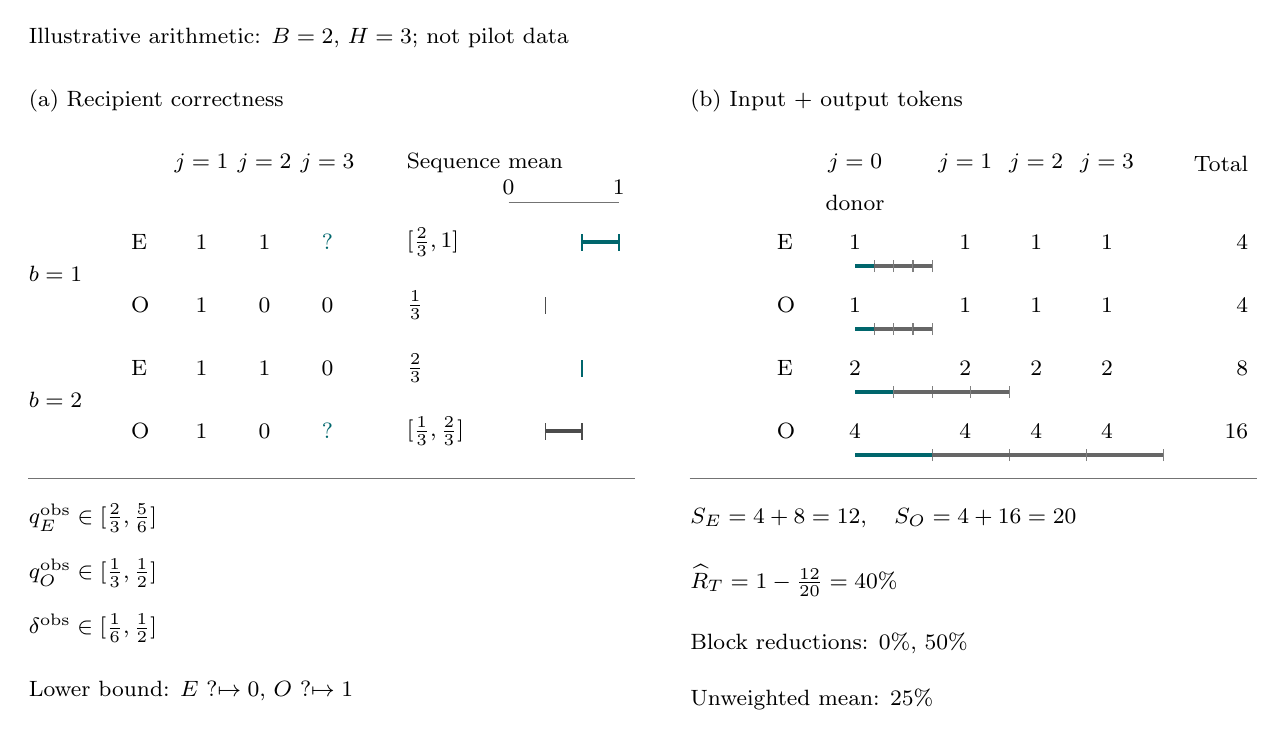
\begin{tikzpicture}[x=1mm,y=1mm,
  every node/.style={font=\fontsize{8.5}{10}\selectfont,inner sep=0pt},
  ealexamplerule/.style={black!55,line width=0.45pt}]
\node[anchor=west] at (0,91) {Illustrative arithmetic: $B=2$, $H=3$; not pilot data};
\node[anchor=west] at (0,83) {(a) Recipient correctness};
\node[anchor=west] at (84,83) {(b) Input + output tokens};
\node at (22,75) {$j=1$}; \node at (30,75) {$j=2$}; \node at (38,75) {$j=3$};
\node[anchor=west] at (48,75) {Sequence mean};
\draw[ealexamplerule] (61,70) -- (75,70);
\node at (61,72) {$0$}; \node at (75,72) {$1$};
\node at (105,75) {$j=0$}; \node at (119,75) {$j=1$};
\node at (128,75) {$j=2$}; \node at (137,75) {$j=3$};
\node[anchor=east] at (155,75) {Total};
\node at (105,70) {donor};
\node[anchor=west] at (0,61) {$b=1$};
\node[anchor=west] at (13,65) {E};
\node[anchor=west] at (95,65) {E};
\node[black,anchor=center] at (22,65) {1};
\node[black,anchor=center] at (30,65) {1};
\node[ealexampleteal,anchor=center] at (38,65) {?};
\node[anchor=west] at (48,65) {$ [\frac{2}{3},1] $};
\draw[ealexampleteal,line width=1.3pt] (70.3333,65) -- (75.0000,65);
\draw[ealexampleteal,line width=.6pt] (75.0000,63.9) -- (75.0000,66.1);
\draw[ealexampleteal,line width=.6pt] (70.3333,63.9) -- (70.3333,66.1);
\node at (105,65) {1};
\node at (119,65) {1};
\node at (128,65) {1};
\node at (137,65) {1};
\node[anchor=east] at (155,65) {4};
\draw[ealexampleteal,line width=1.6pt] (105.000,62) -- (107.450,62);
\draw[black!50,line width=.45pt] (107.450,61.2) -- (107.450,62.8);
\draw[black!60,line width=1.6pt] (107.450,62) -- (109.900,62);
\draw[black!50,line width=.45pt] (109.900,61.2) -- (109.900,62.8);
\draw[black!60,line width=1.6pt] (109.900,62) -- (112.350,62);
\draw[black!50,line width=.45pt] (112.350,61.2) -- (112.350,62.8);
\draw[black!60,line width=1.6pt] (112.350,62) -- (114.800,62);
\draw[black!50,line width=.45pt] (114.800,61.2) -- (114.800,62.8);
\node[anchor=west] at (13,57) {O};
\node[anchor=west] at (95,57) {O};
\node[black,anchor=center] at (22,57) {1};
\node[black,anchor=center] at (30,57) {0};
\node[black,anchor=center] at (38,57) {0};
\node[anchor=west] at (48,57) {$ \frac{1}{3} $};
\draw[black!70,line width=1.3pt] (65.6667,57) -- (65.6667,57);
\draw[black!70,line width=.6pt] (65.6667,55.9) -- (65.6667,58.1);
\node at (105,57) {1};
\node at (119,57) {1};
\node at (128,57) {1};
\node at (137,57) {1};
\node[anchor=east] at (155,57) {4};
\draw[ealexampleteal,line width=1.6pt] (105.000,54) -- (107.450,54);
\draw[black!50,line width=.45pt] (107.450,53.2) -- (107.450,54.8);
\draw[black!60,line width=1.6pt] (107.450,54) -- (109.900,54);
\draw[black!50,line width=.45pt] (109.900,53.2) -- (109.900,54.8);
\draw[black!60,line width=1.6pt] (109.900,54) -- (112.350,54);
\draw[black!50,line width=.45pt] (112.350,53.2) -- (112.350,54.8);
\draw[black!60,line width=1.6pt] (112.350,54) -- (114.800,54);
\draw[black!50,line width=.45pt] (114.800,53.2) -- (114.800,54.8);
\node[anchor=west] at (0,45) {$b=2$};
\node[anchor=west] at (13,49) {E};
\node[anchor=west] at (95,49) {E};
\node[black,anchor=center] at (22,49) {1};
\node[black,anchor=center] at (30,49) {1};
\node[black,anchor=center] at (38,49) {0};
\node[anchor=west] at (48,49) {$ \frac{2}{3} $};
\draw[ealexampleteal,line width=1.3pt] (70.3333,49) -- (70.3333,49);
\draw[ealexampleteal,line width=.6pt] (70.3333,47.9) -- (70.3333,50.1);
\node at (105,49) {2};
\node at (119,49) {2};
\node at (128,49) {2};
\node at (137,49) {2};
\node[anchor=east] at (155,49) {8};
\draw[ealexampleteal,line width=1.6pt] (105.000,46) -- (109.900,46);
\draw[black!50,line width=.45pt] (109.900,45.2) -- (109.900,46.8);
\draw[black!60,line width=1.6pt] (109.900,46) -- (114.800,46);
\draw[black!50,line width=.45pt] (114.800,45.2) -- (114.800,46.8);
\draw[black!60,line width=1.6pt] (114.800,46) -- (119.700,46);
\draw[black!50,line width=.45pt] (119.700,45.2) -- (119.700,46.8);
\draw[black!60,line width=1.6pt] (119.700,46) -- (124.600,46);
\draw[black!50,line width=.45pt] (124.600,45.2) -- (124.600,46.8);
\node[anchor=west] at (13,41) {O};
\node[anchor=west] at (95,41) {O};
\node[black,anchor=center] at (22,41) {1};
\node[black,anchor=center] at (30,41) {0};
\node[ealexampleteal,anchor=center] at (38,41) {?};
\node[anchor=west] at (48,41) {$ [\frac{1}{3},\frac{2}{3}] $};
\draw[black!70,line width=1.3pt] (65.6667,41) -- (70.3333,41);
\draw[black!70,line width=.6pt] (65.6667,39.9) -- (65.6667,42.1);
\draw[black!70,line width=.6pt] (70.3333,39.9) -- (70.3333,42.1);
\node at (105,41) {4};
\node at (119,41) {4};
\node at (128,41) {4};
\node at (137,41) {4};
\node[anchor=east] at (155,41) {16};
\draw[ealexampleteal,line width=1.6pt] (105.000,38) -- (114.800,38);
\draw[black!50,line width=.45pt] (114.800,37.2) -- (114.800,38.8);
\draw[black!60,line width=1.6pt] (114.800,38) -- (124.600,38);
\draw[black!50,line width=.45pt] (124.600,37.2) -- (124.600,38.8);
\draw[black!60,line width=1.6pt] (124.600,38) -- (134.400,38);
\draw[black!50,line width=.45pt] (134.400,37.2) -- (134.400,38.8);
\draw[black!60,line width=1.6pt] (134.400,38) -- (144.200,38);
\draw[black!50,line width=.45pt] (144.200,37.2) -- (144.200,38.8);
\draw[ealexamplerule] (0,35) -- (77,35);
\draw[ealexamplerule] (84,35) -- (156,35);
\node[anchor=west] at (0,30) {$q_E^{\mathrm{obs}}\in [\frac{2}{3},\frac{5}{6}]$};
\node[anchor=west] at (0,23) {$q_O^{\mathrm{obs}}\in [\frac{1}{3},\frac{1}{2}]$};
\node[anchor=west] at (0,16) {$\delta^{\mathrm{obs}}\in [\frac{1}{6},\frac{1}{2}]$};
\node[anchor=west] at (0,8) {Lower bound: $E$ ?$\mapsto 0$, $O$ ?$\mapsto 1$};
\node[anchor=west] at (84,30) {$S_E=4+8=12,\quad S_O=4+16=20$};
\node[anchor=west] at (84,22) {$\widehat R_T=1-\frac{12}{20}=40\%$};
\node[anchor=west] at (84,14) {Block reductions: $0\%$, $50\%$};
\node[anchor=west] at (84,7) {Unweighted mean: $25\%$};
\end{tikzpicture}
\endgroup
